\documentclass[11pt]{article}
\usepackage{amsgen,amsmath,amstext,amsbsy,amsopn,amssymb}
%\usepackage[dvips]{graphicx,color}
\usepackage{graphicx,color}
\usepackage{graphicx,color,bm}
\usepackage{epsfig}
\usepackage{enumerate}
\usepackage{float}

%\setlength{\oddsidemargin}{0.1 in} \setlength{\evensidemargin}{-0.1
%in} \setlength{\topmargin}{-0.6 in} \setlength{\textwidth}{6.5 in}
%\setlength{\textheight}{8.5 in} \setlength{\headsep}{0.75 in}
%\setlength{\parindent}{0 in} \setlength{\parskip}{0.1 in}

\textwidth 6.3in \textheight 8.8in \topmargin -0.5truein
\oddsidemargin .15truein
\parskip .1in
\renewcommand{\baselinestretch}{1.53}  % double spaced


\newcommand{\homework}[9]{
	\pagestyle{myheadings}
	\thispagestyle{plain}
	\newpage
	\setcounter{page}{1}
	\noindent
	\begin{center}
		\framebox{
			\vbox{\vspace{2mm}
				\hbox to 6.28in { {\bf Math531:~Regression - I  \hfill} }
				\vspace{6mm}
				\hbox to 6.28in { {\Large \hfill #1 (#2)  \hfill} }
				\vspace{6mm}
				\hbox to 6.28in { {\it Instructor: #3 \hfill} }
				\hbox to 6.28in { {\it Office hours: #4  \hfill #6}}
				\vspace{2mm}}
		}
	\end{center}
	\markboth{#1}{#1}
	\vspace*{4mm}
}

% ----------------------- MATH -------------------------
\def\av{\boldsymbol a}
\def\bv{\boldsymbol b}
\def\cv{\boldsymbol c}
\def\dv{\boldsymbol d}
\def\ev{\boldsymbol e}
\def\fv{\boldsymbol f}
\def\gv{\boldsymbol g}
\def\hv{\boldsymbol h}
\def\iv{\boldsymbol i}
\def\gv{\boldsymbol j}
\def\kv{\boldsymbol k}
\def\lv{\boldsymbol l}
\def\mv{\boldsymbol m}
\def\nv{\boldsymbol n}
\def\ov{\boldsymbol o}
\def\pv{\boldsymbol p}
\def\qv{\boldsymbol q}
\def\rv{\boldsymbol r}
\def\sv{\boldsymbol s}
\def\tv{\boldsymbol t}
\def\uv{\boldsymbol u}
\def\vv{\boldsymbol v}
\def\wv{\boldsymbol w}
\def\xv{\boldsymbol x}
\def\yv{\boldsymbol y}
\def\zv{\boldsymbol z}
\def\Av{\boldsymbol A}
\def\Bv{\boldsymbol B}
\def\Cv{\boldsymbol C}
\def\Dv{\boldsymbol D}
\def\Ev{\boldsymbol E}
\def\Fv{\boldsymbol F}
\def\Gv{\boldsymbol G}
\def\Hv{\boldsymbol H}
\def\Iv{\boldsymbol I}
\def\Gv{\boldsymbol J}
\def\Kv{\boldsymbol K}
\def\Lv{\boldsymbol L}
\def\Mv{\boldsymbol M}
\def\Nv{\boldsymbol N}
\def\Ov{\boldsymbol O}
\def\Pv{\boldsymbol P}
\def\Qv{\boldsymbol Q}
\def\Rv{\boldsymbol R}
\def\Sv{\boldsymbol S}
\def\Tv{\boldsymbol T}
\def\Uv{\boldsymbol U}
\def\Vv{\boldsymbol V}
\def\Wv{\boldsymbol W}
\def\Xv{\boldsymbol X}
\def\Yv{\boldsymbol Y}
\def\Zv{\boldsymbol Z}
\def\Abf{\mathbf A}
\def\Bbf{\mathbf B}
\def\Cbf{\mathbf C}
\def\Dbf{\mathbf D}
\def\Ebf{\mathbf E}
\def\Fbf{\mathbf F}
\def\Gbf{\mathbf G}
\def\Hbf{\mathbf H}
\def\Ibf{\mathbf I}
\def\Gbf{\mathbf J}
\def\Kbf{\mathbf K}
\def\Lbf{\mathbf L}
\def\Mbf{\mathbf M}
\def\Nbf{\mathbf N}
\def\Obf{\mathbf O}
\def\Pbf{\mathbf P}
\def\Qbf{\mathbf Q}
\def\Rbf{\mathbf R}
\def\Sbf{\mathbf S}
\def\Tbf{\mathbf T}
\def\Ubf{\mathbf U}
\def\Vbf{\mathbf V}
\def\Wbf{\mathbf W}
\def\Xbf{\mathbf X}
\def\Ybf{\mathbf Y}
\def\Jbf{\mathbf J}
\def\Zbf{\mathbf Z}
\def\Am{\mathrm A}
\def\Bm{\mathrm B}
\def\Cm{\mathrm C}
\def\Dm{\mathrm D}
\def\Em{\mathrm E}
\def\Fm{\mathrm F}
\def\Gm{\mathrm G}
\def\Hm{\mathrm H}
\def\Im{\mathrm I}
\def\Gm{\mathrm J}
\def\Km{\mathrm K}
\def\Lm{\mathrm L}
\def\Mm{\mathrm M}
\def\Nm{\mathrm N}
\def\Om{\mathrm O}
\def\Pm{\mathrm P}
\def\Qm{\mathrm Q}
\def\Rm{\mathrm R}
\def\Sm{\mathrm S}
\def\Tm{\mathrm T}
\def\Um{\mathrm U}
\def\mv{\mathrm V}
\def\Wm{\mathrm W}
\def\Xm{\mathrm X}
\def\Ym{\mathrm Y}
\def\Zm{\mathrm Z}
\newcommand{\Ac}{\mathcal{A}}
\newcommand{\Bc}{\mathcal{B}}
\newcommand{\Cc}{\mathcal{C}}
\newcommand{\Dc}{\mathcal{D}}
\newcommand{\Ec}{\mathcal{E}}
\newcommand{\Fc}{\mathcal{F}}
\newcommand{\Gc}{\mathcal{G}}
\newcommand{\Hc}{\mathcal{H}}
\newcommand{\Ic}{\mathcal{I}}
\newcommand{\Jc}{\mathcal{J}}
\newcommand{\Kc}{\mathcal{K}}
\newcommand{\Lc}{\mathcal{L}}
\newcommand{\Mc}{\mathcal{M}}
\newcommand{\Nc}{\mathcal{N}}
\newcommand{\Oc}{\mathcal{O}}
\newcommand{\Pc}{\mathcal{P}}
\newcommand{\Qc}{\mathcal{Q}}
\newcommand{\Rc}{\mathcal{R}}
\newcommand{\Sc}{\mathcal{S}}
\newcommand{\Tc}{\mathcal{T}}
\newcommand{\Uc}{\mathcal{U}}
\newcommand{\Vc}{\mathcal{V}}
\newcommand{\Wc}{\mathcal{W}}
\newcommand{\Xc}{\mathcal{X}}
\newcommand{\Yc}{\mathcal{Y}}
\newcommand{\Zc}{\mathcal{Z}}
\newcommand{\alphav}{\mbox{\boldmath{$\alpha$}}}
\newcommand{\betav}{\mbox{\boldmath{$\beta$}}}
\newcommand{\gammav}{\mbox{\boldmath{$\gamma$}}}
\newcommand{\deltav}{\mbox{\boldmath{$\delta$}}}
\newcommand{\epsilonv}{\mbox{\boldmath{$\epsilon$}}}
\newcommand{\zetav}{\mbox{\boldmath$\zeta$}}
\newcommand{\etav}{\mbox{\boldmath{$\eta$}}}
\newcommand{\iotav}{\mbox{\boldmath{$\iota$}}}
\newcommand{\kappav}{\mbox{\boldmath{$\kappa$}}}
\newcommand{\lambdav}{\mbox{\boldmath{$\lambda$}}}
\newcommand{\muv}{\mbox{\boldmath{$\mu$}}}
\newcommand{\nuv}{\mbox{\boldmath{$\nu$}}}
\newcommand{\xiv}{\mbox{\boldmath{$\xi$}}}
\newcommand{\omicronv}{\mbox{\boldmath{$\omicron$}}}
\newcommand{\piv}{\mbox{\boldmath{$\pi$}}}
\newcommand{\rhov}{\mbox{\boldmath{$\rho$}}}
\newcommand{\sigmav}{\mbox{\boldmath{$\sigma$}}}
\newcommand{\tauv}{\mbox{\boldmath{$\tau$}}}
\newcommand{\upsilonv}{\mbox{\boldmath{$\upsilon$}}}
\newcommand{\phiv}{\mbox{\boldmath{$\phi$}}}
\newcommand{\varphiv}{\mbox{\boldmath{$\varphi$}}}
\newcommand{\chiv}{\mbox{\boldmath{$\chi$}}}
\newcommand{\psiv}{\mbox{\boldmath{$\psi$}}}
\newcommand{\omegav}{\mbox{\boldmath{$\omega$}}}
\newcommand{\Sigmav}{\mbox{\boldmath{$\Sigma$}}}
\newcommand{\Lambdav}{\mbox{\boldmath{$\Lambda$}}}
\newcommand{\Deltav}{\mbox{\boldmath{$\Delta$}}}
\newcommand{\Omegav}{\mbox{\boldmath{$\Omega$}}}
\newcommand{\varepsilonv}{\mbox{\boldmath{$\varepsilon$}}}

\newcommand{\eps}{\varepsilon}
\newcommand{\epsv}{\mbox{\boldmath{$\varepsilon$}}}

\def\1v{\mathbf 1}
\def\0v{\mathbf 0}
\def\Id{\mathbf I} % identity matrix
\newcommand{\ind}[1]{\mathbbm{1}_{\left[ {#1} \right] }}
\newcommand{\Ind}[1]{\mathbbm{1}_{\left\{ {#1} \right\} }}
\newcommand\indep{\protect\mathpalette{\protect\independenT}{\perp}}\def\independenT#1#2{\mathrel{\rlap{$#1#2$}\mkern2mu{#1#2}}}
\newcommand{\QED}{\begin{flushright} {\bf QED} \end{flushright}}
\newcommand{\R}{\mathbb R}
\newcommand{\Real}{\mathbb R}
\newcommand{\C}{\mathbb C}
\newcommand{\E}{\mathbb E}
\newcommand{\sgn}{\mathop{\mathrm{sign}}}
\def\Pr{\mathrm P}
\def\pr{\mathrm P}
\newcommand{\Var}{\mathop{\rm Var}}
\newcommand{\var}{\mathop{\rm Var}}
\newcommand{\Cov}{\mathop{\rm Cov}}
\newcommand{\cov}{\mathop{\rm Cov}}
\newcommand{\Corr}{\mathop{\rm Corr}}
\newcommand{\ang}{\mathop{\rm Angle}}
\newcommand{\tr}{\mathop{\rm trace}}
\newcommand{\proj}{\mathop{\rm Proj}}
\newcommand{\rank}{\mathop{\rm rank}}

\newcommand{\diag}{\mathop{\rm diag}}
\newcommand{\Diag}{\mathop{\rm diag}}
\newcommand{\sk}{\vspace{0.5cm}}
\newcommand{\ds}{\displaystyle}
\newcommand{\mb}{\mbox}
\newcommand{\wh}{\widehat}
\newcommand{\argmin}{\operatornamewithlimits{argmin}}
\newcommand{\argmax}{\operatornamewithlimits{argmax}}

\newcommand{\norm}[1]{\|#1\|}
\newcommand{\abs}[1]{\left\vert#1\right\vert}
\newcommand{\set}[1]{\left\{#1\right\}}

\newcommand{\To}{\longrightarrow}

\def\equalLaw{\stackrel{\mathcal{L}}{=}}
\def\equallaw{\stackrel{\mathcal{L}}{=}}

\def\half{\frac{1}{2}}

\usepackage{caption}

\begin{document}

\begin{title}
	{\Large\bf Homework 5, DATA 556: Due Tuesday, 10/31/2018}
\end{title}

\author{\bf Alexander Van Roijen}

\maketitle

\newpage
Please complete the following:
\begin{enumerate}
\item Problem 1
Let $U \sim $Unif(a, b).
\begin{enumerate}
	\item Use simulations in R (the statistical programming language) to numerically estimate the median and
	the mode of U for a = 0 and b = 2.
	\begin{verbatim}
	set.seed(123)
	n=100000
	binUnif(n,0,2)
		binUnif= function(n,a,b)
		{
		resultsog = runif(n,a,b)
		results = floor(resultsog*10)
		data = data.frame(results)
		vals = seq(a,b,.1)
		p<-ggplot(data=data, aes(x=factor(data[,1]))) +geom_bar(stat="count") + scale_x_discrete(labels=vals)
		p
		#barplot(results,main="whatev",width=0.5)
		print(median(resultsog))
		}
	[1] 0.9987686
	\end{verbatim}
	\begin{figure}[H]
		\centering
		\caption{Mode roughly equivalent across all values of x}
		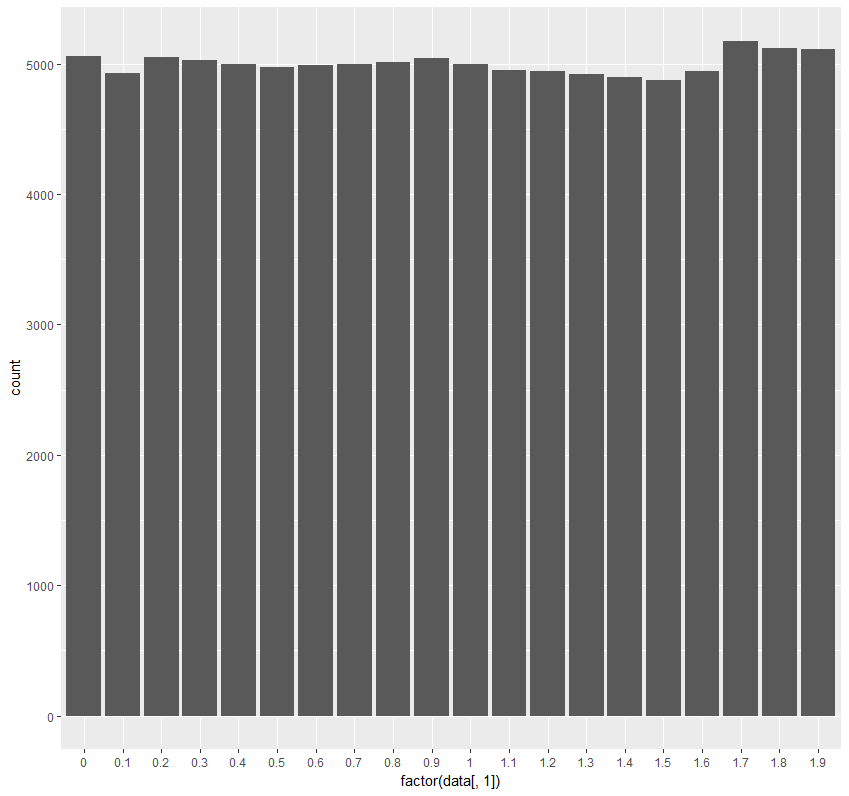
\includegraphics[scale=.6]{Rplot.png}
	\end{figure}
	\item Find the Median and Mode of $U \sim $ Unif(a,b)
	\begin{gather}
	\text{Take the result form above and take the derivative }\\
	f(X|X>a) = F'(X|X>a) = \frac{dF(X|X>a)}{dx} = \frac{F'(x)-F'(a)}{1-F(a)} \text{ with} \frac{dF(a)}{dx} = 0 \\
	=> f(X|X>a) =\frac{f(x)}{1-F(a)}
	\end{gather}
	\item Check that the conditional PDF from (b) is a valid PDF, by showing directly that it is non negative and integrates to 1.
	\begin{gather}
	f(X|X>a) \ge 0 \forall x \text{ as } f(X|X>a) =\frac{f(x)}{1-F(a)} \\
	\text{and we know that } f(x) \ge 0 \forall x \text{ as well as that } 1-F(a) \text{ is a const}
	\\
	\text{Thusly, } f(X|X>a) \ge 0 \forall x \text{ according to these facts}
	\\
	\\
	\text{Now we show } \int_{-\infty}^{\infty} f(X|X>a)dx = 1 \text{ using the fact that } \int_{-\infty}^{\infty} f(x)dx =  = 1 \\
	\int_{-\infty}^{\infty} f(X|X>a)dx = \int_{-\infty}^{a} f(X|X>a)dx + \int_{a}^{\infty} f(X|X>a)dx = \int_{a}^{\infty} f(X|X>a)dx\\
	\text{the above is true as we know $f(X|X>a)$ has no density for x below a}
	\\
	=\int_{a}^{\infty} \frac{f(x)}{1-F(a)}dx = \frac{1}{1-F(a)}\int_{a}^{\infty} f(x)dx \text{ and since we know F is a valid cdf we get }\\
	= \frac{1}{1-F(a)}[1 -F(a)] = 1 \square 
	\end{gather}
\end{enumerate}
\item Problem 2: A circle with a random radius $R \sim Unif(0,1)$ is generated. Let A be its area.
\\
\begin{enumerate}
	\item Use R to simulate mean and variance of A
	\\
	\begin{verbatim}
	> set.seed(123)
	> #this is 2a
	> n=1000000
	> results = runif(n,0,1)
	> counter = 1
	> areas=numeric(0)
	> while(counter<n)
	+ {
	+   areas[counter] = results[counter] * results[counter] * pi
	+   counter= counter + 1
	+ }
	> print(mean(areas))
	[1] 1.045967
	> print(var(areas))
	[1] 0.8775327
	\end{verbatim}
	\item Find the theoretical mean and the variance of A, without first finding the CDF or PDF of A. Compare
	with your numerical results from (a).
	\begin{gather}
	E[A] = \pi E[r^2]\\
	\text{we know r folows Unif(0,1)} => E[r^2] = Var(r) + E[r]^2 = \frac{1}{12} + \frac{1}{2}^2 = \frac{1}{3}\\
	=> E[A] = \frac{\pi}{3} = 1.047198\\
	\var[A] = \var[\pi * r^2] = \pi^2\var[r^2] = \pi^2 * (E[r^4]-E[r^2]^2) = 
	\pi^2 (\int_{0}^{1}r^4 dr -(\frac{1}{3})^2) \\
	= \pi^2 (\frac{1}{5} -\frac{1}{9}) = 0.87729816898 
	\end{gather}
	\item Find the CDF and PDF of A.
	\begin{gather}
	F(x) = P(A \le x) = P(\pi R^2 \le x) = P(R \le \frac{\sqrt{x}}{\sqrt{\pi}})= F(x) = \frac{\sqrt{x}}{\sqrt{\pi}}\\
	f(x) = F'(x) = \frac{1}{\pi} * \frac{d\sqrt{x}}{\sqrt{dx}} = \frac{1}{2\sqrt{x \pi}}
	\\
	\text{with } 0 \le x \le \pi
	\end{gather}
\end{enumerate}
\item A stick of length 1 is broken at a uniformly random point, yielding two pieces. Let X and Y be the lengths
of the shorter and longer pieces, respectively, and let $R = \frac{X}{Y}$ be the ratio of the lengths of X and Y.
\begin{enumerate}
	\item  Use simulations in R (the statistical programming language) to gain some understanding about the distribution of the random variable R. Numerically estimate the expected value of R and $1/R$.
	\begin{verbatim}
	> set.seed(123)
	> n= 1000
	> results = runif(n,0,1)
	> counter = 1
	> xs = numeric(0)
	> ys = numeric(0)
	> while(counter <= n)
	+ {
	+   if(results[counter]>=0.5)
	+   {
	+     ys[counter]=results[counter]
	+     xs[counter] = 1-ys[counter]
	+   }
	+   else
	+   {
	+     xs[counter] = results[counter]
	+     ys[counter] = 1 -xs[counter]
	+   }
	+   counter = counter + 1
	+ }
	> rs = xs/ys
	> print(mean(rs))
	[1] 0.3877773
	> print(mean(1/rs))
	[1] 15.82287
	\end{verbatim}
	\item Find the CDF and PDF of R.\\
	We note that since x is exclusively smaller than y of a unit length stick, then \\
	$0\le X \le 0.5$ and $0.5 \le Y \le 1$ and $X = 1-Y $ and $Y= 1-X$\\
	and that X = min(U,1-U) and Y = max(U,1-U)
	\begin{gather}
	P(R \le r) = P(\frac{X}{Y} \le r) =  P(\frac{X}{(1-X)} \le r) = P(X \le r*(1-X)) = P(X + rX \le r) \\
	= P(X(1+r) \le r) = P(X \le \frac{r}{1+r}) = P(\text{min}(U \text{ or }1-U) \le \frac{r}{1+r}) \\
	= P(U\le \frac{r}{1+r}) + P((1-U) \le \frac{r}{1+r}) + P(U\cap(1-U)\le \frac{r}{1+r}) \text{ by def of OR/union} \\
	= P(U\le \frac{r}{1+r}) + P((1-U) \le \frac{r}{1+r}) + 0 \\
	\text{ the above is true as in the intersect case, both U values cant be realized simultaneously}\\
	\text{(except for when U = .5, but this is a single point in a continuous distribution)}\\
	= P(U\le \frac{r}{1+r}) + P(U \ge 1 - \frac{r}{1+r} ) =  P(U\le \frac{r}{1+r}) + 1 - P(U \le 1 - \frac{r}{1+r} ) \\
	= \frac{r}{1+r} + 1 - (1-\frac{r}{1+r}) = \frac{r}{1+r} + 1 - \frac{1}{1+r} \\
	=> F(r) = \frac{2r}{1+r} \\
	=> f(r) = (1+r)^{-1} \frac{d}{dr}(2r)+ 2r\frac{d}{dr}(1+r)^{-1}=(1+r)^{-1}(2)+ 2r(-1)(1+r)^{2} \\
	= \frac{2+2r - 2r}{(1+r)^{2}} = f(r) = \frac{2}{(1+r)^{2}}
	\end{gather}
	\item Find the expected value of R (if it exists).
	\begin{gather}
	E[R] = \int_{-\infty}^{\infty}r*f(r)dr = \int_{-\infty}^{\infty}\frac{2r}{(1+r)^{2}}dr = \int_{0}^{1}\frac{2r}{(1+r)^{2}}dr = 2(\frac{1}{1+r} + \log(1+r))\Big|_0^1\\ 
	= 2((\frac{1}{2} + \log(2)) - (\frac{1}{1} + \log(1))) = 2((\frac{1}{2} + \log(2)) - 1) = 2\log(2) - 1 = 0.3862944
	\end{gather}
	\item Find the expected value of 1/R if it exits.
	\begin{gather}
	E[\frac{1}{R}] = \int_{-\infty}^{\infty}\frac{1}{r}*f(r)dr = \int_{-\infty}^{\infty}\frac{2}{r(1+r)^{2}}dr = \int_{0}^{1}\frac{2}{r(1+r)^{2}}dr = 2*(\frac{1}{r+1} + \log(r) - log(1+r)\Big|_0^1)\\ 
	\text{However, this can not be evaluated as the log of zero is undefined}
	\end{gather}
\end{enumerate}
\item Let $U_1,...,U_n$ be i.i.d. $Unif(0,1)$, and $X = max(U_1,...,U_n)$.
\begin{enumerate}
	\item What is the PDF of X?
	\begin{gather}
		\text{CDF} = P(X \le x) = P(U_1 \le x , ... , U_n \le x) = P(U_1 \le x) *  ... * P(U_n \le x) \text{ since i.i.d}\\
		=> \text{CDF} = x*x*x...*x = x^n => \text{ PDF } = \frac{dF}{dx} = n*x^{n-1} \text{ with } 0 \le x \le 1
	\end{gather}
	\item what is the $E[X]$
	\begin{gather}
		\int_{-\infty}^{\infty}x*f(x) = \int_{0}^{1}x*f(x) = \int_{0}^{1}x*n*x^{n-1} = \int_{0}^{1}n*x^{n} =\frac{n}{n+1}*(1^n) - 0 = \frac{n}{n+1}
	\end{gather}
	\item R simulation results / approx
	\begin{verbatim}
		> #4c
		> set.seed(123)
		> n=10
		> runplenty=10000
		> og = runif(n,0,1)
		> counter=1
		> result= numeric(0)
		> while(counter<=runplenty)
		+ {
		+   og = runif(n,0,1)
		+   result[counter]=max(og)
		+   counter= counter+1
		+ }
		> print(mean(result))
		[1] 0.9091953
		> print(n/(n+1))
		[1] 0.9090909
	\end{verbatim}
\end{enumerate}
\item 
\begin{enumerate}
	\item Find $P(X < Y)$ for X $\sim N(a, b), Y \sim N(c, d)$ with X and Y independent
	\begin{gather}
	\Var(X-Y) = \Var(X) + Var(Y) = b^2 + d^2\\
	E[X-Y] = E[X] - E[Y] = a - c\\
	=>	P(X<Y) = P(X-Y < 0) \sim N(a-b,c^2 + d^2) \text{ determined via hint}\\
		= \int_{-\infty}^{0} \frac{1}{\sqrt{2\pi} \sigma} e ^ {\frac{(x-\mu)^2}{2\sigma ^2}} \text{ Where } \sigma = \sqrt{c^2 + d^2} \text{ and } \mu = a-b
	\end{gather}
	\item R simulation
	\begin{verbatim}
		#5b
		> set.seed(123)
		> n= 1000000
		> resultsx = rnorm(n,0,1)
		> resultsy = rnorm(n,1,5)
		> trueResults = rnorm(n,-1,sqrt(26))
		> counter = 1
		> numCorr=0
		> numCorr2=0
		> results=numeric(0) 
		> while(counter<=n)
		+ {
		+   if(resultsx[counter]<resultsy[counter])
		+   {
		+     numCorr = numCorr + 1
		+   }
		+   if(trueResults[counter]<0)
		+   {
		+     numCorr2 = numCorr2 + 1
		+   }
		+   counter= counter+1
		+ }
		> print(numCorr/n)
		[1] 0.576969
		> print(numCorr2/n)
		[1] 0.577764
	\end{verbatim}
\end{enumerate}
\item The heights of men in the United States are normally distributed with mean 69.1 inches and standard deviation
2.9 inches. The heights of women are normally distributed with mean 63.7 inches and standard deviation 2.7 inches. Let x be the average height of 100 randomly sampled men, and y be the average height
of 100 randomly sampled women.
\begin{enumerate}
	\item What is the distribution of x - y?
	\begin{gather}
		\text{Similar to 5, except now we need to calculate the expected value and variance over the 100 samples}\\
		E[x-y] = E[\frac{1}{n}\sum_{n=1}^{100} x_n-y_n] =\frac{1}{n}\sum_{n=1}^{100} E[X_n] - E[y_n] =\frac{1}{n}\sum_{n=1}^{100} (69.1-63.7) = \frac{1}{n} n*(69.1-63.7) \\
		\text{we got this from the distributions of the random variables given}\\
		=> E[x-y] = 5.4\\
		\Var[x-y] = \Var[\frac{1}{n}\sum_{n=1}^{100} x_n-y_n] =\frac{1}{n^2}\Var[\sum_{n=1}^{100} x_n-y_n] \text{ from independence we get}\\
		= \frac{1}{n^2}\sum_{n=1}^{100} (\Var[x_n]+\Var[y_n]) = \frac{1}{n^2}\sum_{n=1}^{100} (2.9^2+2.7^2) = \frac{1}{n^2}n (15.7) = \frac{1}{100}(15.7) \\
		=> \Var[x-y] = \sqrt{\frac{15.7}{100}}^2\\
		=>
		x-y \sim N(5.4,\sqrt{\frac{15.7}{100}})
	\end{gather}
	\item R monte carlo simulations 
	\begin{verbatim}
		> set.seed(123)
		> n=100
		> numTrials=100000
		> counter=1
		> diffRes = numeric(0)
		> while(counter<numTrials)
		+ {
		+   resultsx = rnorm(n,69.1,2.9)
		+   resultsy = rnorm(n,63.7,2.7)
		+   diffRes[counter] = mean(resultsx)-mean(resultsy)
		+   counter = counter + 1
		+ }
		> resultCalc = rnorm(n,5.4,sqrt(15.7/n))
		> print(mean(diffRes))
		[1] 5.400457
		> print(mean(resultCalc))
		[1] 5.381992
		> print(var(diffRes))
		[1] 0.1570096
		> print(var(resultCalc))
		[1] 0.1590042
	\end{verbatim}
	Clearly, we can see that these make sense intuitively.\\
	\item What is the probability that a man is taller than a randomly sampled woman?\\
	let X be the RV for a man sampled and Y be a RV for a woman sampled
	\begin{gather}
		\text{Note, that the } P(X-Y<0) = P(X<Y) => P(X>Y) = 1 - P(X<Y) = 1 -P(X-Y<0) \\
		\text{we can assume this as the } P(X=Y) = 0\\
		\text{We know } X-Y \sim N(5.4,\sqrt{15.7})\\
		=> 1-P(X-Y<0) = 1 - 0.08646693 = .9135331
	\end{gather}
	Note, the value above was derived using dbinom from R
\end{enumerate}
\item Suppose we have a RV Y such that $Y \sim \text{Binom}(n=5,p = \theta)$
\begin{enumerate}
	\item Using Bayes Rule to determine $P(\theta | y)$ in terms of $\theta_i$
	\begin{gather}
		 P(\theta | y) = \frac{P(Y | \theta_i) * P(\theta_i)}{P(Y)} = \frac{\binom{5}{y} \theta_i^y(1-\theta_i)^{5-y} * \frac{1}{11}}{P(Y)}
		 \\
		 \text{Now with the law of total probability, we get}\\
		 = \frac{\binom{5}{y} \theta_i^y(1-\theta_i)^{5-y} * \frac{1}{11}}{\sum_{i=0}^{11}\binom{5}{y} \theta_i^y(1-\theta_i)^{5-y} * \frac{1}{11}} = \frac{\frac{1}{11}\binom{5}{y} \theta_i^y(1-\theta_i)^{5-y}}{\binom{5}{y} \frac{1}{11}\sum_{i=0}^{11} \theta_i^y(1-\theta_i)^{5-y}} = \frac{ \theta_i^y(1-\theta_i)^{5-y}}{\sum_{i=0}^{11} \theta_i^y(1-\theta_i)^{5-y}}
	\end{gather}
	\item \& (c)
	The previous graphics make complete sense. In particular, notice that the end points are the edge cases of p = 0 and p = 1. In either case, you either need there to be all failures, or all successes, and is thus 0 probability or 1 depending on the y.
	Further, its interesting to note the symmetric nature of this distribution due to the binomial nature and  $\theta$ and $1-\theta$ relationship
\end{enumerate}
\item a) Starting from independent uniform random variables (U $\sim$ Unif(0, 1)), devise an algorithm to generate independent samples from a Logistic distribution, having density
\begin{gather}
	f(x) = \frac{e^{-x}}{(1+e^{-x})^2} => F(x) = (1+e^{-x})^{-1}\\
	=> \text{let } F(x) = u \text{ we want to solve for x in terms of you to find  } F^{-1} \\
	\frac{1}{1+e^{-x}} = u => \frac{1}{u} = 1+e^{-x} => \frac{1-u}{u} = e^{-x} => \log(\frac{1-u}{u}) = -x => F^{-1}(X) = \log(\frac{u}{1-u})
\end{gather}
b) R simulations
\begin{verbatim}
> set.seed(123)
> n=100000
> unifVals = runif(n,0,1)
> invert = log(unifVals/(1-unifVals))
> res = (invert<3 & invert>2)
> print(sum(res == TRUE))
[1] 7077
> print(sum(res==TRUE)/n)
[1] 0.07077
\end{verbatim}
\end{enumerate}

\end{document}
